\documentclass{article}
\usepackage[utf8]{inputenc}
\usepackage{stmaryrd}
\usepackage{amsthm}
\usepackage{amssymb}
\usepackage{amsmath}
\usepackage{tikz}
\usepackage{hyperref}
\usepackage[ruled,vlined,linesnumbered]{algorithm2e}
\newtheorem{ex}{Example}
\title{Two Dimensional Picture Languages: \\ Tiling Systems, Domino Systems and Weighted Finite Automata}
\author{Benedikt Lüken-Winkels }
\date{September 2020}

\begin{document}

\maketitle

\section*{Introduction}
This report provides an overview and a summary of the works of Gimmarresi and Restivo \cite{DBLP:reference/hfl/GiammarresiR97} and Culik and Kari \cite{DBLP:conf/mfcs/CulikK93} on two-dimensional languages, especially focussing on Tiling Systems, Domino Systems and Weighted Finite Automata.






\section{Tiling Systems}
The basic idea of a tiling system is to use the ability of finite automata to recognize a string language by projecting a local language in the two-dimensional world. Therefore the local language can be obtained from a finite set $\Theta$ of square \textit{tiles} of size $2\times2$. Then a two-dimensional language is `tiling recognizable`, if it can be projected from the local picture language.


A tiling system $\mathcal{T}$ is defined as a 4-tuple $\mathcal{T} =\{\Sigma, \Gamma, \Theta, \pi \}$. Let $\Sigma$ and $\Gamma$ be finite alphabets. A language $L \subseteq \Sigma^{**}$ is tiling recognizable, if there is a local language $L' \subseteq \Gamma^{**}$ that can be obtained exactly from tiles taken from the finite set of tiles $\Theta$ over the alphabet $\Gamma \cup \{\#\}$ and a projection $\pi: \Theta \rightarrow \Gamma$. When $L'$ can be obtained from $\Theta$ it can be written as $L' = L(\Theta)$. A computational approach on verifying the locality of $L'$ is to scan a picture from $L'$ with a $2\times2$ window and checking, if every tile is included in $\Theta$.

The recognition of a Language $L$ by a tiling system $\mathcal{T}$ can be written as $L=L(\mathcal{T})$, when $L$ is a projection of some local language. and $L \in \mathcal{L}(TS)$ ($L$ lies in the family of two-dimensional languages recognizable by tiling systems).

\paragraph{Example 1} Let $\Sigma = \{a\}$ be a one-letter alphabet and let $L$ be the language of all pictures over $\Sigma$ with 3 rows. \\ \textit{Claim:} Language $L$ is tiling recognizable.

$$Let\ \Theta = 
\left\{
\begin{array}{c}
\begin{array}{|cc|}
 \hline
 \# & \# \\
 \# & 1 \\
 \hline
\end{array},
\begin{array}{|cc|}
 \hline
 \# & \# \\
 1 & 1 \\
 \hline
\end{array},
\begin{array}{|cc|}
 \hline
 \# & \# \\
 1 & \# \\
 \hline
\end{array}\vspace{3mm}\\
\begin{array}{|cc|}
 \hline
 \# & 1 \\
 \# & 2 \\
 \hline
\end{array},
\begin{array}{|cc|}
 \hline
 1 & 1 \\
 2 & 2 \\
 \hline
\end{array},
\begin{array}{|cc|}
 \hline
 1 & \# \\
 2 & \# \\
 \hline
\end{array}\vspace{3mm}\\
\begin{array}{|cc|}
 \hline
 \# & 2 \\
 \# & 3 \\
 \hline
\end{array},
\begin{array}{|cc|}
 \hline
 2 & 2 \\
 3 & 3 \\
 \hline
\end{array},
\begin{array}{|cc|}
 \hline
 2 & \# \\
 3 & \# \\
 \hline
\end{array}\vspace{3mm}\\
\begin{array}{|cc|}
 \hline
 \# & 3 \\
 \# & \# \\
 \hline
\end{array},
\begin{array}{|cc|}
 \hline
 3 & 3 \\
 \# & \# \\
 \hline
\end{array},
\begin{array}{|cc|}
 \hline
 3 & \# \\
 \# & \# \\
 \hline
\end{array}

\end{array}\right\}$$
Then a picture $p \in L(\Theta)$ can look like this:
$$
\begin{array}{|ccccccc|}
 \hline
 \# & \# & \#& \#& \#& \# & \#\\
 \# & 1 & 1& 1& 1& 1& \# \\
 \# & 2 & 2& 2& 2& 2& \#\\
 \# & 3 & 3& 3& 3& 3& \#\\
 \# & \# & \#& \#& \# & \#& \#\\
 \hline
\end{array}
$$
Using the previously explained method a $2\times2$ window traversing $p$ will always contain a tile from $\Theta$. Now with $\pi$ being defined as $\pi(1) = \pi(2) = \pi(3) = a$, one can see, that $L$ is \textit{tiling recognizable}, so $L \in \mathcal{L}(TS)$.$\qed$\\

This approach works for languages with any number of rows, with a corresponding size of $\Gamma$, since for each row there has to be a dedicated symbol in the alphabet to keep track of the number of rows in each picture from $L' = L(\Theta)$.


\subsection{Closure Properties}

\paragraph{Projection} Let $\Sigma_1$ and $\Sigma_2$ be finite alphabets and $\rho : \Sigma_1 \rightarrow \Sigma_2$ a projection. If $L_1 \subseteq \Sigma_1^{**}$ is tiling recognizable, then $L_2 = \rho(L_1)\ (L_2\subseteq \Sigma_2^{**})$ is too. 
Let $\mathcal{T}_1 = (\Sigma_1, \Gamma, \Theta,\pi_1)$ be recognizing tiling system of $L_1$ and $\mathcal{T}_2 = (\Sigma_2, \Gamma, \Theta,\pi_2)$. Now if $\pi_2$ is defined as $\pi_2 = \rho \circ \pi_1 : \Gamma \rightarrow \Sigma_2$, one can see, that $L_2$ is recognized by $\mathcal{T}_2$. Therefore $L_1,L_2 \in \mathcal{L}(TS)$.

$\Rightarrow$ $\mathcal{L}(TS)$ is closed under projection.

\paragraph{Row and column concatenation} Let $L_1$ and $L_2$ be picture languages over an alphabet $\Sigma$ and let $L = L_1 \varominus L_2$ be the language corresponding to the row concatenation of $L_1$ and $L_2$. Furthermore let $\mathcal{T}_1 = (\Sigma, \Gamma_1, \Theta_1, \pi_1)$ and $\mathcal{T}_2 = (\Sigma, \Gamma_2, \Theta_2, \pi_2)$ be tiling systems for $L_1$ and $L_2$. In a tiling system $\mathcal{T}=(\Sigma, \Gamma, \Theta, \pi)$ for $L$ with $\Gamma = \Gamma_1 \cup \Gamma_2$, $\Theta$ has to contain 
\begin{itemize}
 \item[] each tile from $\Theta_1$ without its bottom borders 
 $$\Theta_1'=\left\{\ 
 \begin{array}{|cc|}
 \hline
 a_1 & b_1 \\
 c_1 & d_1 \\
 \hline
 \end{array}
 \ |\  
 \begin{array}{|cc|}
 \hline
 a_1 & b_1 \\
 c_1 & d_1 \\
 \hline
 \end{array} \in \Theta_1\ and\ c_1,d_1 \neq \#
 \ \right\},
 $$
 \item[] each tile from $\Theta_2$ without its upper borders
  $$\Theta_2'=\left\{\ 
 \begin{array}{|cc|}
 \hline
 a_1 & b_1 \\
 c_1 & d_1 \\
 \hline
 \end{array}
 \ |\  
 \begin{array}{|cc|}
 \hline
 a_1 & b_1 \\
 c_1 & d_1 \\
 \hline
 \end{array} \in \Theta_2\ and\ a_1,b_1 \neq \#
 \ \right\}  \textrm{ and}
 $$
 \item[] connecting (gluing) tiles
 $$\Theta_{12}=\left\{\ 
 \begin{array}{|cc|}
 \hline
 \# & a_1 \\
 \# & a_2 \\
 \hline
 \end{array},
  \begin{array}{|cc|}
 \hline
 b_1 & \# \\
 b_2 & \# \\
 \hline
 \end{array},
  \begin{array}{|cc|}
 \hline
 c_1 & d_1 \\
 c_2 & d_2 \\
 \hline
 \end{array}
 \ |\                    
 \begin{array}{c}
\begin{array}{|cc|}     % Begin Theta 1
 \hline
 \# & a_1 \\
 \# & \# \\
 \hline
 \end{array},
  \begin{array}{|cc|}
 \hline
 b_1 & \# \\
 \# & \# \\
 \hline
 \end{array},
  \begin{array}{|cc|}
 \hline
 c_1 & d_1 \\
 \# & \# \\
 \hline
 \end{array} \in \Theta_1\\
\begin{array}{|cc|}     % Begin Theta 2
 \hline
 \# & \# \\
 \# & a_2 \\
 \hline
 \end{array},
  \begin{array}{|cc|}
 \hline
 \# & \# \\
 b_2 & \# \\
 \hline
 \end{array},
  \begin{array}{|cc|}
 \hline
 \# & \# \\
 c_2 & d_2 \\
 \hline
 \end{array} \in \Theta_2
 \end{array}
 \ \right\}.
 $$ 
\end{itemize}
Then $\Theta = \Theta_1 \cup \Theta_2 \cup \Theta_{12}$ and $\pi : \Gamma \rightarrow \Sigma$ maps the tile's symbols corresponding to their 'origins':
$$\forall a \in \Gamma, \hspace{5mm} \pi(a) = \left\{d
\begin{array}{cc}
 \pi_1(a) & \textrm{if } a\in \Gamma_1 \\
 \pi_2(a) & \textrm{if } a\in \Gamma_2 \backslash \{\Gamma_1 \cap \Gamma_2\} \\
\end{array}\right.$$


For the \textit{column concatenation} $L = L_1 \varobar L_2 $ there is a similar approach, but in this case with $\Theta_1$ including all but the right and $\Theta_2$ all but the left bordered tiles. The 'gluing' set of tiles $\Theta_{12}$ corresponds to the columns where the pictures are concatenated.

$\Rightarrow$ $\mathcal{L}(TS)$ is closed row and column concatenation.

\paragraph{Row and column closure} For a tiling system $(\Sigma, \Gamma, \Theta, \pi)$ for $L^{*\varominus}$, two different tiling systems can be used to build $\Gamma$ as the union of sets of tiles without upper and lower borders and the set of gluing tiles, as shown above. With the same technique a tiling system for $L^{*\varobar}$ can be defined.


$\Rightarrow$ $\mathcal{L}(TS)$ is closed row and column closure operations.



\paragraph{Union and intersection} Let $L_1$ and $L_2$ be picture languages over an alphabet $\Sigma$ and let $L = L_1 \cup L_2$ be the language corresponding to the union of $L_1$ and $L_2$. Furthermore let $(\Sigma, \Gamma_1, \Theta_1, \pi_1)$ and $(\Sigma, \Gamma_2, \Theta_2, \pi_2)$ be tiling systems for $L_1$ and $L_2$, respectively. A tiling system $(\Sigma, \Gamma, \Theta, \pi)$ for $L$ has $\Gamma = \Gamma_1 \cup \Gamma_2$ with $\Theta = \Theta_1 \cup \Theta_2$. The projection $\pi$ is defined corresponding to $\pi_1$ and $\pi_2$ as above.

$(\Sigma, \Gamma, \Theta, \pi)$ for the language $L= L_1 \cap L_2$ uses as local alphabet $\Gamma$ a subset of $\Gamma_1 \times \Gamma_2$ to identify tiles that occur in both $\Theta_1$ and $\Theta_2$. Two symbols that map to the same symbol in $\Sigma$ create a pair, that belongs to $\Gamma$: 
$$(a_1, a_2) \in \Gamma \Leftrightarrow \pi_1(a_1) = \pi_2(a_2)$$
Now $\Theta$ consists of tiles, where these pairs of symbols correspond to their origins:
 $$\Theta=\left\{\ 
 \begin{array}{|cc|}
 \hline
 (a_1,a_2) & (b_1, b_2) \\
 (c_1, c_2) & (d_1, d_2) \\
 \hline
 \end{array}
 \ |\  
 \begin{array}{|cc|}
 \hline
 a_1 & b_1 \\
 c_1 & d_1 \\
 \hline
 \end{array} \in \Theta_1\ and\
  \begin{array}{|cc|}
 \hline
 a_2 & b_2 \\
 c_2 & d_2 \\
 \hline
 \end{array} \in \Theta_2\
 \ \right\},
 $$


$\Rightarrow$ $\mathcal{L}(TS)$ is closed under union and intersection.

\paragraph{Complement} Let $\Sigma = \{a,b\}$ and let $L = \{p \in \Sigma^{**} | p = s\varominus s \textrm{ wheres is a square}\}$ be the language of rectangles with identical upper and lower halves. If $L \in \mathcal{L}(TS)$, then there is a local $L'$ over an alphabet $\Gamma$ from which $L$ can be obtained by projection. In general $|\Sigma| \leq |\Gamma|$, as seen in previous examples. Now, let $L_n$ be the language of rectangles with identical squares as upper and lower halves of size $n$ and $L'_n$ the local language over $\Gamma$ that can be projected to $L_n$ by $\pi$. There are $|\Sigma|^{n^2}$ possible pictures of $L_n$ and $|\Gamma|^{2n}$ possible $n$-th and $(n+1)$-th rows in pictures of $L'_n$. So for a large $n$ there will be two pictures $p' = s_p' \varominus s_p''$ and $q' = s_q' \varominus s_q''$ in $L'_n$ with identical $n$-th and $(n+1)$-th rows and projections $p = s_p \varominus s_p$ and $q = s_q \varominus s_q$ in $L_n$ with $s_p \neq s_q$. Since the $n$-th and $(n+1)$-th rows are identical $\Theta$ contains tiles that allow to obtain the picture $v' = s_p' \varominus s_q''$ with $\pi(v') = s_p \varominus s_q$, creating a picture not in $L_n$. 


The complement of $L$ $^cL$ can be written as $^cL = L_1 \cup L_2$, the union of the language with rectangles of size $\neq (2n,n)$ and the language of rectangles of size $(2n,n)$ with different top and bottom halves. $L_1$ is recognizable by a tiling system, that creates a rectangle using descending stairs, two by one, starting in the top left corner and then missing the last square on the bottom right. $L_2$ can be decomposed in several languages that are recognized by tiling systems using the same technique as for $L_1$.\\
Now one can see, that $L \notin \mathcal{L}(TS)$, while $^cL \in \mathcal{L}(TS)$.


$\Rightarrow$ $\mathcal{L}(TS)$ is not closed under complement.

\paragraph{Rotation} To obtain a tiling system for the rotation $L^R$ of a language $L$ with tiling system $(\Sigma, \Gamma, \Theta, \pi)$, the tiles in $\Theta$ are rotated. $(\Sigma, \Gamma, \Theta^R, \pi)$ recognizes $L^R$.


$\Rightarrow$ $\mathcal{L}(TS)$ is closed under rotation.












\section{Domino Systems}
In domino systems, the definition of the local language is altered and called hv-local language. Instead of using $(2\times2)$-tiles, horizontal and vertical dominoes of sizes $(1,2)$ and $(2,1)$ define the new set of tiles. A two-dimensional language $L \subseteq \Gamma^{**}$ is hv-local, if there exists a finite set of dominoes $\Delta$ over $\Gamma \cup \{\#\}$ that exactly 'produces' $L$. 
A domino system is a 4-tuple $\mathcal{D}=(\Sigma, \Gamma, \Delta, \pi)$ where $\Sigma$ and $\Gamma$ are finite alphabets, $\Delta$ is the set of dominoes over $\Gamma \cup \{\#\}$ and $\pi: \Gamma \rightarrow \Sigma$. 

\paragraph{Example 2} As seen later, the family of domino systems $\mathcal{L}(DS) = \mathcal{L}(TS)$, so the language $L$ of all pictures over $\Sigma = \{a\}$ with three rows from example 2, can be is recognizable by domino systems:

$$\Delta = \left\{ 
\begin{array}{c}
 \begin{array}{|c|}
  \hline
  \#\\
  \#\\
  \hline
 \end{array},
\begin{array}{|c|}
  \hline
  \#\\
  1\\
  \hline
 \end{array},
 \begin{array}{|cc|}
  \hline
  1 & 1\\
  \hline
 \end{array},
 \begin{array}{|cc|}
  \hline
  \# & \#\\
  \hline
 \end{array},
 \begin{array}{|cc|}
  \hline
  1 & \#\\
  \hline
 \end{array},
\end{array}
\right\}$$









\paragraph{Proposition 1} $L$ is an $hv$-local language, then $L$ is a local language, too. 

Let $L=L(\Delta)$ and $\Theta$ be a finite set of tiles, that consist of dominoes from $\Delta$. To show, that also $L=L(\Theta)$, let $p\in L(\Theta)$ and $q \in L(\Delta)$. As defined, in $p$ any ($1\times2$) sub-block $B_{1,2}(\widehat{p})$ and ($2\times1$) sub-block in $B_{1,2}(\widehat{p})$ is included in $\Delta$. So $p \in L(\Theta)$.

Any ($2\times2$) sub-block $B_{2,2}(\widehat{q})$ of $q$ is a tile from $\Theta$. Since those tiles are made of dominoes from $\Delta$, $q \in L(\Delta)$.$\qed$ \newline
There are local languages that are not $hv$-local, so the converse of this proposition does not hold.

\subsection{$\mathcal{L}(TS) = \mathcal{L}(DS)$}
The inclusion of domino systems in tiling systems $\mathcal{L}(TS) \subseteq \mathcal{L}(DS)$ follows from proposition 1. For the other direction $\mathcal{L}(DS) \subseteq \mathcal{L}(TS)$ can be shown by proving, that for a local language $L$ over $\Sigma$, there exists an $hv$-local language $L'$ over $\Gamma$ and a mapping $\pi:\Gamma \rightarrow \Sigma$ with $L=\pi(L')$ that allows to project pictures from $L'$ to $L$:


Let $L=L(\Theta)$ over $\Sigma$ with $\Theta$ being the set of tiles over $\Sigma \cup \{\#\}$. $L'$ with $L=L(\Delta)$ can be obtained by creating a set of dominoes $\Delta$ over a larger alphabet $\Gamma$ such that its elements only 'fit' into one another, if certain conditions hold. Therefore $\Gamma = \Theta$, so $\Delta$ consists of dominoes of two tiles:

$$\Delta=\left\{\ 
\begin{array}{|cc|cc|}
 \hline
 a_1 & a_2 & b_1 & b_2 \\
 a_3 & a_4 & b_3 & b_4 \\
 \hline
\end{array},
\begin{array}{|cc|}
 \hline
 c_1 & c_2 \\
 c_3 & c_4 \\
 \hline
 d_1 & d_2 \\
 d_3 & d_4 \\
 \hline
\end{array}\ |\ 
\begin{array}{c}

\begin{array}{|cc|}
 \hline
 a_1 & a_2 \\
 a_3 & a_4 \\
 \hline
\end{array},
\begin{array}{|cc|}
 \hline
 b_1 & b_2 \\
 b_3 & b_4 \\
 \hline
\end{array},
\begin{array}{|cc|}
 \hline
 c_1 & c_2 \\
 c_3 & c_4 \\
 \hline
\end{array},
\begin{array}{|cc|}
 \hline
 d_1 & d_2 \\
 d_3 & d_4 \\
 \hline
\end{array} \in \Gamma\\
\text{and } a_2=b_1, a_4=b_3,c_3=d_1,c_4=d_2
\end{array}
\ \right\}$$

with the mapping 
\begin{align*}
 \pi:\ & \Gamma \rightarrow \Sigma\\
 & \begin{array}{|cc|}
     \hline
     a_1 & a_2 \\
     a_3 & a_4 \\
     \hline
    \end{array}\rightarrow a_1
\end{align*}
a picture $p'$ in the $hv$-local language $L'=L(\Delta)$ consists of $(2\times 2)$ tiles, where each tile is mapped to  the symbol in the upper left corner. The condition for the dominoes in $\Delta$, that their symbols have to match where  the two tiles are glued together then leads to a mapping, where each tile of a picture $p \in L = L(\Theta)$ is represented as a construct of $(4\times 4)$ symbols, made of 3 dominoes from $\Delta$ as seen in the following example (the '$\dots$' represent 'don't cares'):

$$\underbrace{
  \begin{array}{|cc|}
   \hline
   \# & \# \\
   \# & a \\
   \hline
   \# & a \\
   \# & a \\
   \hline
  \end{array}\ ,
  \begin{array}{c}
   \begin{array}{|cc|cc|}
   \hline
   \# & \# & \# & \# \\
   a & a & \dots & \dots \\
   \hline
  \end{array}\ ,\\  \\
  \begin{array}{|cc|cc|}
   \hline
   a & a & \dots & \dots \\
   a & \dots & \dots & \dots \\
   \hline
  \end{array}
  \end{array}}_{\in \Delta}\rightarrow
  \underbrace{\begin{array}{|cc|}
   \hline
   \# & \# \\
   \# & a \\
   \hline
  \end{array}}_{\in \Theta}
$$
The example shows another special property of this contruction: Tiles in $\Delta$ with a border symbol $\#$ in the upper left corner are entirely used as a border symbol, so, as for all the other tiles in $\Delta$ the remaining symbols are used for correct positionioning.

Formally, to show that $\pi(L') = L$, let $p' \in L'$ and $q \in B_{2,2}(p')$ be a $(2\times 2)$ sub-picture of $p'$.
$$q=\begin{array}{|cc|cc|}
     \hline
     a_1 & b_1 & b_1 & b_2 \\
     c_1 & d_1 & d_1 & d_2 \\
     \hline
     c_1 & d_1 & d_1 & d_2 \\
     c_2 & d_3 & d_3 & d_4 \\
     \hline
    \end{array}
$$
With all the symbols in $q$ from $\Sigma \cup \{\#\}$ and because of the definition of $\Delta$, the four tiles are in $\Theta$, so 
$$\pi(q) = 
\begin{array}{|cc|}
 \hline
 a_1 & b_1 \\
 c_1 & d_1\\
 \hline
\end{array}\in \Theta
$$


For the converse a picture $p' \in L'$ to a corresponding $p \in L$ is defined by mapping each symbol $s$ at with coordinates $(i,j)$ of $p$ to a $(2\times 2)$ tile, where the upper left symbol is $s$ and tile looks like 
$$\begin{array}{|cc|}
\hline
s & p(i, j+1)\\
p(i+1,j) & p(i+1, j+1)\\
\hline
\end{array}
$$
By definition of $\pi$: $\pi(p')=p$. Therefore $L=\pi(L')$. $\qed$









\newpage
\section{Weighted Finite Automata}

A WFA describes a grey-scale picture by focussing on the relation between parts and subparts of the image. Therefore the image is recursively partitioned into four quadrants which can be addressed by a quadtree. \\
Let $\Sigma = \{ (0,0), (0,1), (1,0),(1,1)\}$ be the alphabet for words $w \in \Sigma^*$ which form a path through the quadtree to either find a $node$, i.e. a subsquare in the image, or a $leaf$, i.e. the smallest unit in the image, a $pixel$ for images with finite resolution. A finite finite-resolution image usually consists of $(2^n \times 2^n)$ pixels whith a fixed $n$, while a multi-resolution image is a collection of several images, with $n=0,1,\dots$ . Then the addressing scheme works as seen in figure \ref{fig:addr}, starting from the bottom left corner with the entire image having the address $\varepsilon$.
\begin{figure}[ht]
\centering
\input{addressing} 
\caption{Example for addressing subsquares in images for WFA}
\label{fig:addr}
\end{figure}

Let $f: \Sigma^* \rightarrow \mathbb{R}$ be the greyness function that assigns a greyness value to a subsquare. To describe an rgb color picture, three images are necessary.

A function $f: \Sigma^* \rightarrow \mathbb{R}$ is average preserving, if 
$$f(w) = \frac{1}{4}[f(w(0,0)) + f(w(0,1)) + f(w(1,0)) + f(w(1,1))] $$
for each $w \in \Sigma^*$. This means, that the average greyness of the subsquare with the address $w$ of a picture $p$ is equal to the average greyness of its subsquares. 

A weighted finite automaton is a 5-tuple $\mathcal{A}= (Q, \Sigma, f, \alpha, \beta)$, with 
\begin{itemize}
 \item $Q$ the finite set of states,
 \item $\Sigma$ the finite alphabet to form the addresses of the subsquares\\($\Sigma = \{(0,0), (0,1),(1,0),(1,1)\}$),
 \item $f: Q \times \Sigma \times Q \rightarrow [-\infty, \infty]$ the function assigning weights to the transitions in the automaton,
 \item $\alpha: Q \rightarrow [-\infty, \infty]$ the initial distribution and
 \item $\beta \rightarrow [-\infty, \infty]$ the final distribution on the greyness scale.
\end{itemize}

If $f(p,a,q) \neq 0$, $(p,a,q)$ is a transition.
Now the distribution function $\delta: Q \times \Sigma^* \rightarrow [-\infty, \infty]$ is defined as 
\begin{align*}
\delta(q,\varepsilon) &= \alpha(q),\ \forall q\in Q \\
\delta(q,wa)&= \sum_{p\in Q} \delta(p,w) \cdot f(p,a,q),\ \forall p\in Q, w\in \Sigma^* \text{ and }a\in \Sigma
\end{align*}
With this, the WFA $\mathcal{A}$ defines the function $\phi_{\mathcal{A}}:\Sigma^* \rightarrow [-\infty, \infty]$, which returns the greyness value of a subsquare with a given word (address) $w \in \Sigma^*$, by summing up the initial distribution of the starting state, the final distribution of the final state and the weights of the transitions for each path in the automaton that forms the input word $w$:
$$\phi_{\mathcal{A}}(w) = \sum_{q_0,\dots,q_n \in Q} \alpha(q_0) \cdot f(q_0,a_1,q_1) \cdot \dots \cdot f(q_{n-1}, a_n, q_n ) \cdot \beta(q_n)$$
In other words, the sum of the weights on all paths leading from state $p$ to $q$ corresponds to the effect, the state $q$ has on the image.

A WFA $\mathcal{A}$ is average preserving, iff 

$$\forall p \in Q:\ \sum_{a\in \Sigma, q\in Q} (f(p,a,q) \cdot \beta(q)) = 4 \cdot \beta(p)$$
so the sum of the greyness values (distribution) after all possible state transitions from state $p$ is equal to four times its final distribution value $\beta(p)$. Then, if $\mathcal{A}$ is average perserving, $\phi_{\mathcal A}$ is average preserving.

\subsection{Encoding an image with a WFA}
The encoding of an image with a WFA means being able to reconstruct the image up to a certain resolution. A $2^k$ by $2^k$ resolution would create a quadtree of height $k$, where all values are on one level. Then, propagating towards the root each node is assigned the average value of its children.

The encoding algorithm generates a WFA $\mathcal A$ and $\phi_\mathcal A$ for a given distribution function $\phi$, such that $\phi_\mathcal A = \phi$. The goal is to find an automaton with as few states as possible. There are several ways to improve the algorithm, when used in practise. By introducing an error margin $e$, the amount of transitions can be reduced. If the transition weight lies below a certain value it is set to 0 and is no longer taken into account. The result is, that the encoded image is no longer equal to image to be encoded, but is still similar (depending on the size of $e$). In addition the size of the automaton decreases.

Algorithm \ref{algo:wfa} shows the encoding procedure of an image given by $\phi$ to a WFA $\mathcal{A}$ and the corresponding $\phi_\mathcal A$.
\newline


\begin{algorithm}[H]
\label{algo:wfa}
\SetAlgoLined
\label{algo:add}
\SetKwInOut{Input}{input}
\SetKwRepeat{Do}{do}{while}
\Input{Distribution function $\phi$ for the given image}
$N \gets 0$\\
$i \gets 0$\\
$\beta(q_0) \gets \phi(\varepsilon)$\\
$\gamma(q_0) \gets \varepsilon$\\
\Do{$i\leq N$}{
    $w\gets \gamma(q_i)$\\
    \ForEach{$a\in \{(0,0),(0,1), (1,0), (1,1) \}$}{
        Find $c:=c_0,\dots,c_N$ such that $\phi_{wa}=c_0\phi_0+\dots+c_N\phi_N$ (for each $a$), where $\phi_j$ corresponds to the subsquare of the $j$-th state $q_j$ ($\phi_{\gamma(q_j)}$)\\
        
        \uIf{c exists}{
            \For{$j=0,\dots,N$}{
                $f(q_i,a,q_j)\gets c_j$
            }
        }\Else{
            $\gamma(q_{N+1}) \gets wa$\\
            $\beta(q_{N+1}) \gets \phi(wa)$ \\
            $f(q_i, a, q_{N+1}) \gets 1$ \\
            $N \gets N + 1$
        }
    }
    $i\gets i+1$
}
$\alpha(q_0) \gets 1$\\
\For{$j = 1,\dots, N$}{
    $\alpha(q_j) \gets 0$
}


\caption{Construct WFA $\mathcal{A}$ and $\phi_\mathcal{A}$ for image given by $\phi$}
\end{algorithm}

\paragraph{Example 3} Figure \ref{fig:automaton} shows the automaton, that can be used to generate the image shown in figure \ref{fig:img}. Using the WFA-encoding algorithm (algorithm \ref{algo:wfa}) this automaton is created in as follows:
\begin{enumerate}
 \item $q_0$ is assigned to the entire square $\varepsilon$ and  $\beta(q_0):= 0.5$.
 \item Now with $w = \varepsilon$, iterate over the subsquares $\{(0,0),(0,1), (1,0), (1,1) \}$ and try to find $c = c_0,\dots,c_N$.
\begin{enumerate}
  \item $\varepsilon 00:$ For $\phi_{\varepsilon00} = c_0\phi_0 $ $c_0$ gets the value $1.25 \Rightarrow$ $f(q_0,00,q_0):= 1.25$
  \item $\varepsilon 01:$ For $\phi_{\varepsilon01} = c_0\phi_0 $ $c_0$ gets the value $1 \Rightarrow$ $f(q_0,01,q_0):= 1$
  \item $\varepsilon 10:$ For $\phi_{\varepsilon10} = c_0\phi_0 $ $c_0$ gets the value $1\ \Rightarrow$ $f(q_0,10,q_0):= 1$
  \item $\varepsilon 11:$ For $\phi_{\varepsilon11} = c_0\phi_0 $ $c_0$ gets the value $0.5\ \Rightarrow$ $f(q_0,11,q_0):= 0.5$
 \end{enumerate}

 
 
\item $\alpha(q_0) := 1$
\end{enumerate}

\begin{figure}[ht]
$$\renewcommand\arraystretch{1.3}\begin{array}{|c|c|}
 \hline
 \frac{1}{4} & \frac{1}{2} \\
 \hline
 \frac{3}{4} & \frac{1}{2} \\
 \hline
\end{array}$$
\caption{Example image with greyscale}
\label{fig:img}
\end{figure}

\begin{figure}[ht]
 \centering
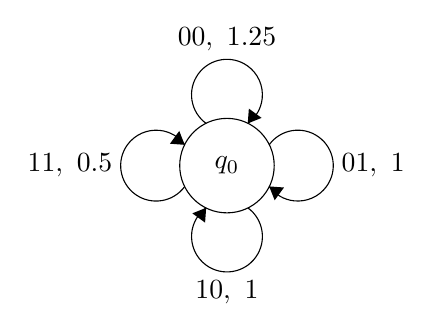
\begin{tikzpicture}[scale=0.2]
\tikzstyle{every node}+=[inner sep=0pt]
\draw [black] (37.7,-21.6) circle (3);
\draw (37.7,-21.6) node {$q_0$};
\draw [black] (36.377,-18.92) arc (234:-54:2.25);
\draw (37.7,-14.35) node [above] {$00,\mbox{ }1.25$};
\fill [black] (39.02,-18.92) -- (39.9,-18.57) -- (39.09,-17.98);
\draw [black] (40.38,-20.277) arc (144:-144:2.25);
\draw (44.95,-21.6) node [right] {$01,\mbox{ }1$};
\fill [black] (40.38,-22.92) -- (40.73,-23.8) -- (41.32,-22.99);
\draw [black] (39.023,-24.28) arc (54:-234:2.25);
\draw (37.7,-28.85) node [below] {$10,\mbox{ }1$};
\fill [black] (36.38,-24.28) -- (35.5,-24.63) -- (36.31,-25.22);
\draw [black] (35.02,-22.923) arc (-36:-324:2.25);
\draw (30.45,-21.6) node [left] {$11,\mbox{ }0.5$};
\fill [black] (35.02,-20.28) -- (34.67,-19.4) -- (34.08,-20.21);
\end{tikzpicture}
\caption{Automaton to generate the image in figure \ref{fig:img}}
\label{fig:automaton}
\end{figure}


\newpage
\nocite{*}
\bibliography{sources.bib}
\bibliographystyle{plain}
\end{document}
 
 
 
 
 
 
 
 
 
 
 
 
 
 
 
 
 
 
 
 
 
 
 
 
 
 
 
 
 
 
 
 
 
